\documentclass{article}

\usepackage{graphicx}
\usepackage{tikz}
\usepackage{tikzsymbols}
\usetikzlibrary{calc,patterns,shapes.geometric}
\pagestyle{empty}
\usepackage[margin=0pt]{geometry}
\geometry{papersize={14in,12in}}

\def\centerarc[#1](#2)(#3:#4:#5){\draw[#1] ($(#2)+({#5*cos(#3)},{#5*sin(#3)})$) arc (#3:#4:#5);}

\begin{document}
	\begin{figure}
		\centering
		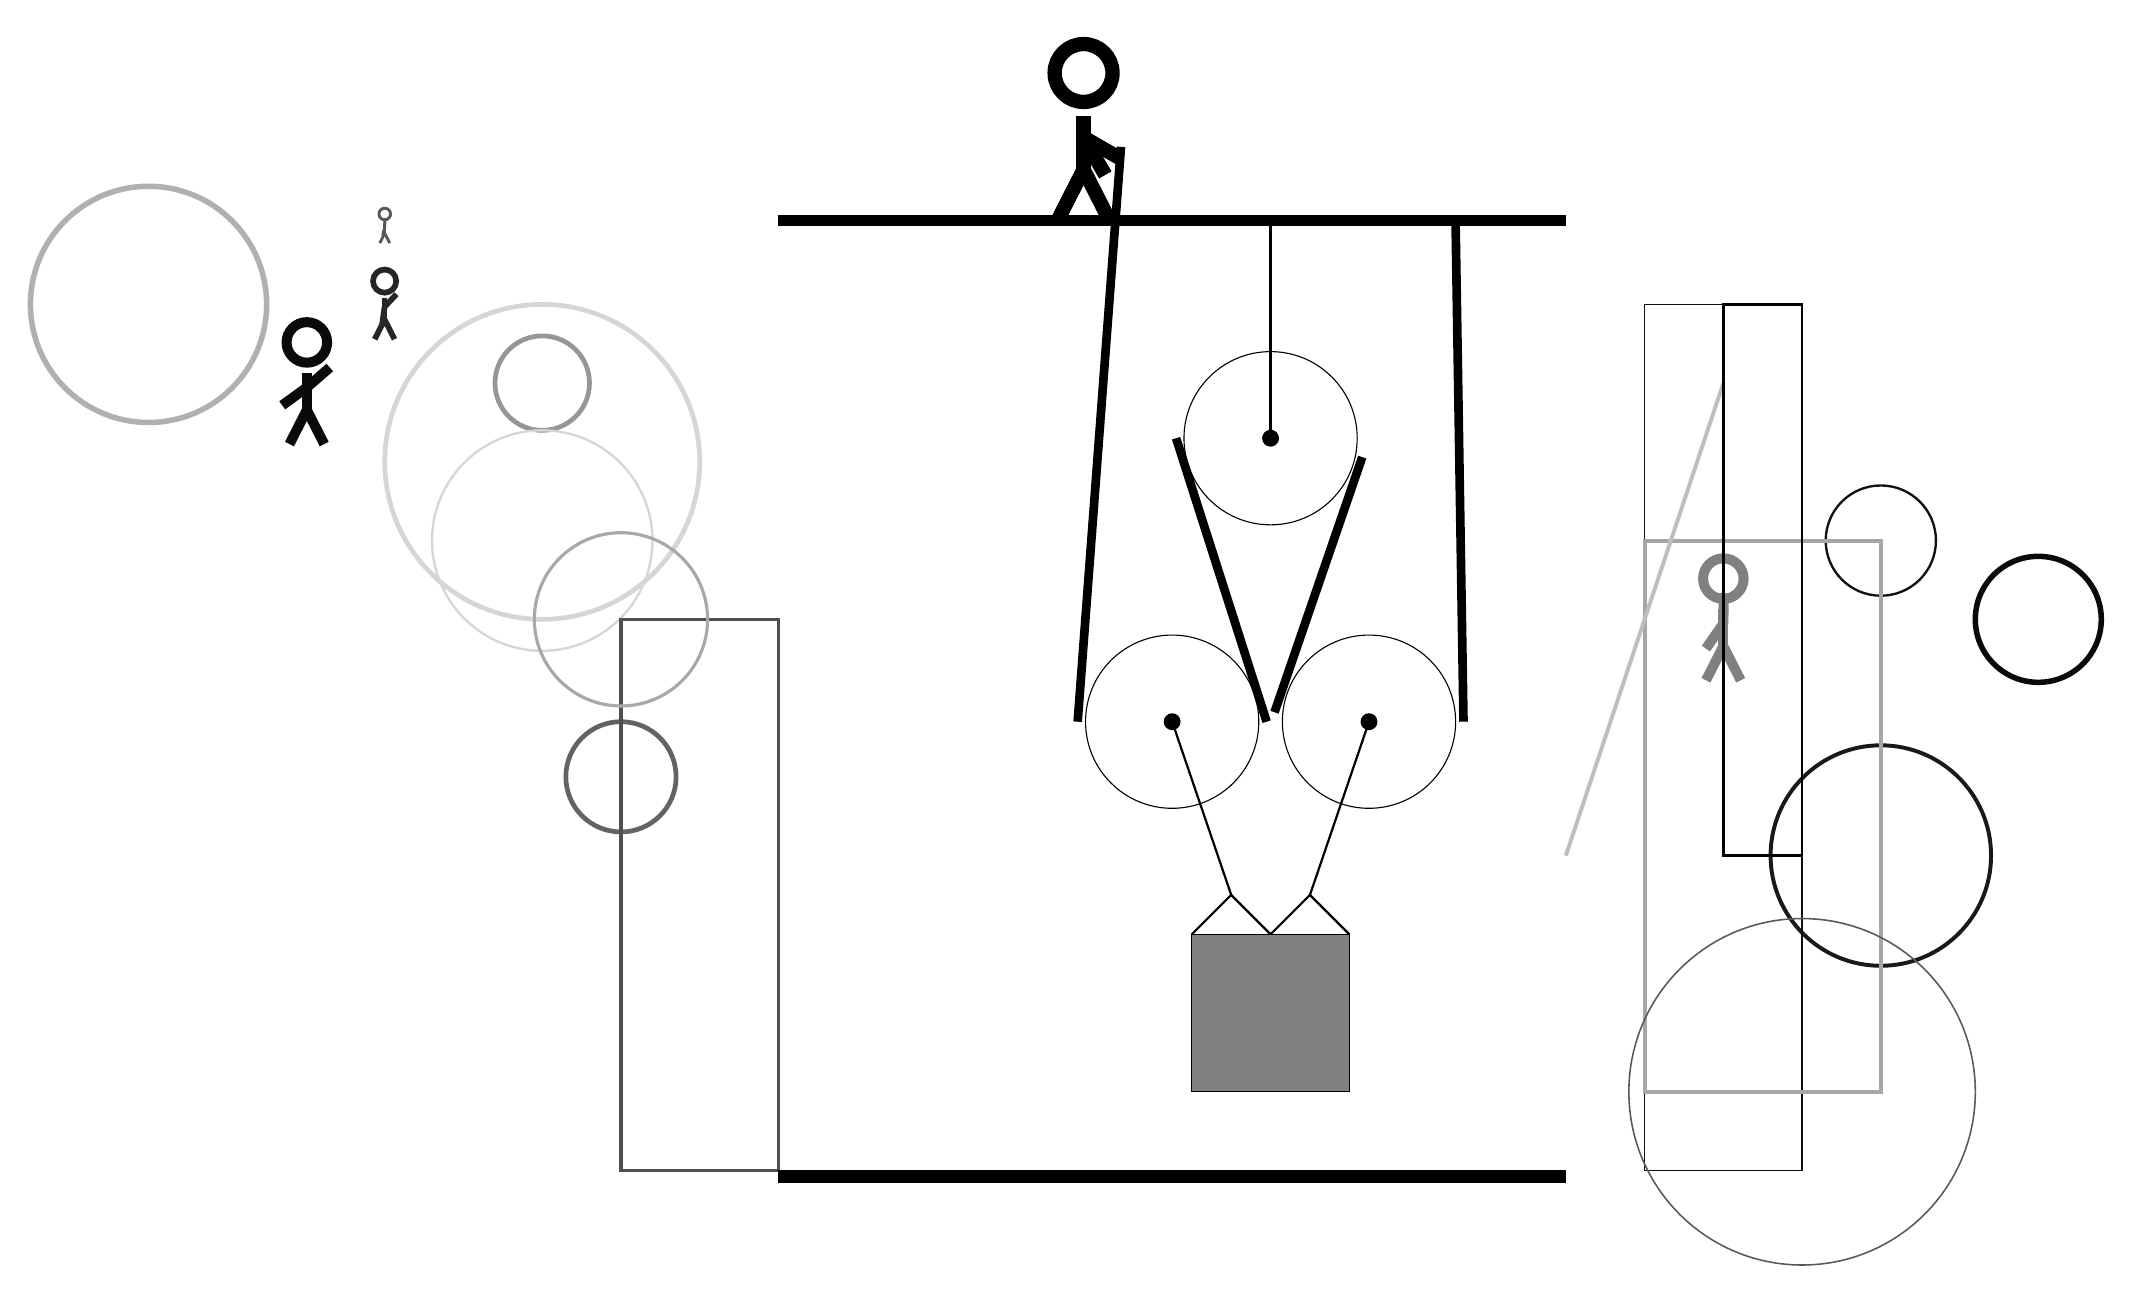
\begin{tikzpicture}
			%%%%% START %%%%%
			
			\draw[fill=black] (-4, 9) rectangle (6, 9.125);
			
			\draw (1, 2.7) circle (1.1);
			\draw[fill=black] (1, 2.7) circle (0.1);
			
			\draw (2.25, 6.3) circle (1.1);
			\draw[fill=black] (2.25, 6.3) circle (0.1);
			\draw[thick] (2.25, 6.3) -- (2.25, 9);
			
			\draw (3.5, 2.7) circle (1.1);
			\draw[fill=black] (3.5, 2.7) circle (0.1);
			
			\draw[thick] (3.5, 2.7) -- (2.75, 0.5);
			\draw[thick] (1, 2.7) -- (1.75, 0.5);
			\draw[thick]  (1.25, 0) -- (1.75, 0.5) -- (2.25, 0);
			\draw[thick]  (2.25, 0) -- (2.75, 0.5) -- (3.25, 0);
			\draw[fill=black!50] (1.25, 0) rectangle (3.25, -2);
			
			\draw[line width=1.1mm] (0.35, 10) --  (-0.2, 2.7);
			\centerarc[line width=1.1mm](1, 2.7)(180:360:1.2000000000000002);
			\draw[line width=1.1mm] (2.2, 2.7) -- (1.05, 6.3);
			\centerarc[line width=1.1mm](2.25, 6.3)(-20:180:1.2000000000000002);
			\draw[line width=1.1mm](3.414, 6.06) -- (2.3, 2.82);
			\centerarc[line width=1.1mm](3.5, 2.7)(160:360:1.2000000000000002);
			\draw[line width=1.1mm](4.7, 2.7) -- (4.6, 9);
			
			\node at (-0.07, 10.2) {\Strichmaxerl[10][120][-30]};
			
			\draw [line width=0.6mm, color=black!41](-7, 7) circle (0.6);
			
			\node[line width=0.6mm, color=black!85] at (-9, 8) {\Strichmaxerl[4][82][47]};
			\draw [line width=0.6mm, color=black!16](-7, 6) circle (2.0);
			\draw[line width=0.2mm, color=black!25] (8, 8) rectangle (8, 7);
			\draw [line width=0.5mm, color=black!90](10, 1) circle (1.4);
			
			\draw[line width=0.2mm, color=black!94] (7, 8) rectangle (9, -3);
			\draw [line width=0.3mm, color=black!93](10, 5) circle (0.7);
			\draw [line width=0.7mm, color=black!31](-12, 8) circle (1.5);
			\draw [line width=0.6mm, color=black!61](-6, 2) circle (0.7);
			\draw[line width=0.5mm, color=black!35] (7, -2) rectangle (10, 5);
			\node[line width=0.6mm, color=black!50] at (8, 4) {\Strichmaxerl[7][55][89]};
			\draw [line width=0.2mm, color=black!65](9, -2) circle (2.2);
			\node[line width=0.5mm, color=black!96] at (-10, 7) {\Strichmaxerl[7][36][41]};
			
			\draw[line width=0.5mm, color=black!26](8, 7) -- (6, 1);
			\draw [line width=0.7mm, color=black!96](12, 4) circle (0.8);
			\draw [line width=0.3mm, color=black!16](-7, 5) circle (1.4);
			
			\node[line width=0.4mm, color=black!66] at (-9, 9) {\Strichmaxerl[2][76][89]};
			
			\draw[line width=0.3mm, color=black!100] (8, 8) rectangle (9, 1);
			\draw[line width=0.4mm, color=black!69] (-4, -3) rectangle (-6, 4);
			\draw [line width=0.4mm, color=black!34](-6, 4) circle (1.1);
			
			\draw[fill=black] (-4, -3) rectangle (6, -3.15);
			
			%%%%% END %%%%%
		\end{tikzpicture}
	\end{figure}	
\end{document}